%!TEX program = xelatex
%!TEX builder = latexmk
% or can be latexmk texify
%!TEX option = 
% -shell-escape -8bit % For minted package
%!TEX root = ...
\documentclass[10pt,a4paper,twocolumn]{article} % titlepage表示标题单独页
\usepackage[noindent]{ctex} % ctex套用英文标题格式 (建议在英文论文混排中文时使用) ,
% ctexcap套用中文格式 (等同于\documentclass{ctexart}) 
% \renewcommand{\figurename}{图}
% \renewcommand{\tablename}{表}
% \renewcommand{\contentsname}{目录}
% \renewcommand\refname{参考文献}
% \renewcommand{\thefigure}{\chinese{figure}} % 将图片计数改为汉字数字
% \renewcommand{\thetable}{\chinese{table}} % 将表格计数改为汉字数字
\usepackage[top=0.75in,bottom=0.75in,left=0.75in,right=0.75in]{geometry} % 页边距设置
% \usepackage{multicol}页面内多行包
\usepackage[CJKbookmarks]{hyperref} % 给pdf文档添加互动式链接和书签
% \userpackage{wrapfig} % 图文绕排
% \usepackage{xeCJK} % to get my Chinese name
% \setCJKmainfont{SimSun}
% \usepackage[parfill]{parskip} % 增加段间行距
\usepackage{amsmath,amssymb,esint} % 数学公式类宏包;最末为积分符号拓展
\allowdisplaybreaks[0]% 允许多行公式间换页, 用//*表示不允许换页
\numberwithin{equation}{section} % 公式编号包含章节
\usepackage{bm} % 加粗 (用于vector) 
\usepackage{mathrsfs} % mathscr font
% \usepackage{textcomp} % 符号包, 不能用于数学模式, 建议不要和SIunits混用
% \usepackage[squaren]{SIunits} % 科学单位包, 可以用于数学模式
% (为了统一不要和textcomp混用) , squaren选项消除和amssymb的冲突
\usepackage{siunitx} % 淘汰掉上面这个宏包吧, 现在用的是
% \num{123}, \si{kg.m/s^2}, 
% \si{\electronvolt\per\square\clight}, \SI{123}{\micro\metre}
\usepackage{extarrows} % 长箭头, 长等号etc.
\usepackage{graphicx} % 插图宏包
% \usepackage{picinpar} % 图文绕排
\usepackage{array} % 表格宏包
% \usepackage{longtable} % 长表格宏包
\usepackage{multirow} % 多行合并的表格宏包
% \usepackage{booktabs} % 表格线宏包
\usepackage{braket} % 狄拉克符号

% \usepackage[basic,box,gate,oldgate,ic,optics,physics]{circ} % 电路图宏包
% \usepackage[normalem]{ulem} % 下划线, 删除线等宏包, 参数表示不修改\emph{}格式
% \usepackage{mychemistry} % 化学宏包, 包含mhchem和chemfig
\usepackage[version=3]{mhchem} % 化学宏包, 包含mhchem和chemfig
% \usepackage[symbol]{footmisc} % 脚注拓展, 选项表示用符号做脚注记号
% \usepackage{listings} % 代码段宏包
% \lstset{numbers=left,frame=shadowbox,%
% basicstyle=\ttfamily, commentstyle=\fontseries{lc}\selectfont\itshape, %
% columns=fullflexible, breaklines=true, escapeinside={(*@}{@*)}}
% \usepackage{minted} % 具有 Python 支持的代码宏包

% \renewcommand*{\vec}[1]{\bm{#1}} % 矢量的格式, 这里是加粗
\newcommand{\dif}{\,\mathrm d}
\newcommand\mi{\mathrm{i}}
\newcommand\e{\mathrm{e}} % 定义数学模式中常用的正体字符
\newcommand\Y{\mathrm{Y}}
\newcommand\cc{\mathrm{c.c.}}
\DeclareMathOperator{\Imag}{Im}
% \bibliographystyle{unsrt}
\begin{document}
\title{原子分子物理笔记}
\author{吕铭 Lyu Ming}
\maketitle
\tableofcontents
\section{原子的电子谱线结构} % (fold)
\label{sec:1st_principle}
\subsection{单电子原子的薛定谔方程} % (fold)
\label{sub:single_ele}
薛定谔方程如
\begin{equation}
	\left[-\frac{\hbar^2}{2\mu}\nabla^2 - 
	\frac{Ze^2}{4\pi\varepsilon_0 r}\right]\psi(\vec r)
	= E\psi(\vec r)
\end{equation}
本征函数 $H\psi_{nlm} = E_n\psi_{nlm}$
\begin{align}
	& \psi_{nlm}(\vec r) = R_{nl}(r) \Y_{lm}(\theta,\phi) \\
	& E_n = -\frac{Z^2}{2}\mu c^2\alpha^2\frac 1{n^2} \\
	& \alpha = \frac{e^2}{4\pi\varepsilon_0\hbar c} \approx \frac 1{137}
\end{align}
% subsection single_ele (end)
\subsection{精细结构修正} % (fold)
\label{sub:fin_str}
相对论效应和场论引入 $H = H_0 + H_1' + H_2' + H_3'$
\begin{align}
	% & H = H_0 + H' = H_0 + H_1' + H_2' + H_3' \\
	& H_0 = \frac{p^2}{2m} - \frac{Z e^2}{4\pi\varepsilon_0 r} \\
	& H_1' = -\frac{p^4}{8m^3c^2} 
	&\mbox{相对论动能}\\
	& H_2' = \frac 1{2m^2c^2} \frac 1r\frac{\dif V}{\dif r}\vec L\cdot\vec S \
	&\mbox{自旋轨道耦合}\\
	& H_3' = \frac{\pi\hbar^2}{2m^2c^2}\left(
	\frac{Ze^2}{4\pi\varepsilon_0}\right)\delta(\vec r)
	&\mbox{Darwin 项}
\end{align}
各向产生的谱线结构:
\begin{itemize}
	\item $H_1'$: 不同 $l$ 的精细结构分裂
	\begin{align}
		\Delta E_1 &= \braket{\psi_{nlm}|H_1'|\psi_{nlm}} \\
		&= -E_n\left(\frac{Z\alpha}{n}\right)^2
		\left(\frac 34 - \frac{n}{l+1/2}\right)
	\end{align}
	\item $H_2'$: 相同 $l$ 的精细结构分裂
	\begin{align}
		\Delta E_2 &= \braket{\psi_{nlmm_s}|H_1'|\psi_{nlmm_s}} \\
		&= \frac{\hbar^2}{2}\langle \xi(r) \rangle 
		\left[j(j+1) - l(l+1) - \frac 34\right]
	\end{align}
	\begin{equation}
		\langle \xi(r) \rangle = -\frac{2E_n}{\hbar^2}
		\frac{(Z\alpha)^2}{2nl(l+1/2)(l+1)}
	\end{equation}
	\item $H_3'$: 只影响 $l = 0$ 的结果, 即
	\begin{equation}
		\Delta E_3 = \braket{\psi_{n00}|H_3'|\psi_{n00}} 
		= -E_n\frac{(Z\alpha)^2}{n}
	\end{equation}
	\item 总的结果恰好与 $l$ 无关 (不计 Lamb 位移)
	\begin{equation}
		\Delta E_{nj} = E_n\left(\frac{Z\alpha}{n}\right)^2
		\left(\frac{n}{j+1/2} - \frac 34\right)
	\end{equation}
\end{itemize}
% subsection fin_str (end)
\subsection{Lamb 位移} % (fold)
\label{sub:lamb_shift}
原子量子场论的真空涨落, 使得 $^2\mathrm S_{1/2}$ 和 $^2\mathrm P_{1/2}$ 
之间有 $\SI{E3}{MHz}$ 的分裂
% subsection lamb_shift (end)
\subsection{超精细结构} % (fold)
\label{sub:hperfine_splitting}
来自于电子角动量 $\vec J$ 与核自旋 $\vec I$ 的相互作用: 
\begin{equation}
\begin{aligned}
	H_{\mathrm{hfs}} = & A_{\mathrm{hfs}}\vec I\cdot\vec J \\
	& + B_{\mathrm{hfs}}\frac{3(\vec I\cdot\vec J)^2 + 3(\vec I\cdot\vec J)/2
	- \vec I^2\vec J^2}{2I(2I-1)J(2J-1)}
\end{aligned}	
\end{equation}
第一项来自磁偶极, 第二项来自电四极. 忽略第二项: 
\begin{equation}
	\Delta E = A \left[F(F+1) - I(I+1) - J(J+1)\right]
\end{equation}
如\ce{^{87}Rb} 中 $A > 0$
% subsection hperfine_splitting (end)
% section 1st_principle (end)
\section{原子与电磁场相互作用} % (fold)
\label{sec:int_with_emf}
一般的电荷与电磁场的哈密顿量: 
\begin{align}
	H = \sum_\alpha \frac 12 m_\alpha\vec v_\alpha^2
	+\frac{\varepsilon_0}2\int\dif^3\vec r\left[\vec E^2 + c^2\vec B^2\right]
\end{align}
此外还包含包含守恒量: 
\begin{align}
	& \vec P = \sum_\alpha m_\alpha\vec v_\alpha + 
	\varepsilon_0\int\dif^3 r\, \vec E\times\vec B \\
	& \vec J = \sum_\alpha\vec r_\alpha\times m_\alpha\vec v_\alpha + 
	\varepsilon_0\int\dif^3 r\, \vec r \times\left[\vec E\times\vec B\right]
\end{align}
势场的定义和规范变换: 
\begin{align}
	&\vec B = \nabla\times\vec A \\
	&\vec E = -\frac{\partial}{\partial t}\vec A - \nabla\vec U 
\end{align}
\begin{align}
	\vec A &\to \vec A' = \vec A + \nabla\chi \\
	U &\to U' = U - \frac{\partial \chi}{\partial t}
\end{align}
纵场 ($\nabla\times \vec V_\parallel = 0$) 
与横场 $(\nabla\cdot\vec V_\perp = 0$) 分开, 可写为
\begin{align}
	&H = T + V_c + H_t  \\
	&T = \sum_\alpha\frac{1}{2m_\alpha}
	\left[\vec P_\alpha - q_\alpha\vec A_\perp(\vec r_\alpha)\right]^2\\
	&V_c = \frac 12\sum_{\alpha\neq\beta} \frac{1}{4\pi\varepsilon_0}
	 \frac{q_\alpha q_\beta}{|\vec r_\alpha - \vec r_\beta|} + 
	 \sum_\alpha E_{\mathrm{self}} \\
	&H_t = \frac{\varepsilon_0}2\int\dif^3\vec r
	 \left[\vec E_\perp^2 + \vec B^2\right]
\end{align}
选取库伦规范时, $\vec A_\perp = \vec A$. 

引入常磁场 $\vec B$ 时, 可以得到轨道磁矩与磁场作用
\footnote{与讲义不同, 本整理中凡涉及自旋, $L, S, I$ 等都表示单位自旋, 不包含 $\hbar$ 量纲.}: 
\begin{equation}
	H_{\mathrm{int}} = \frac{e\hbar}{2m} \vec B\cdot\vec L 
	= \mu_B\vec B\cdot\vec L
\end{equation}
\subsection[Land\'e g 因子]{Land\'e $g$ 因子} % (fold)
\label{sub:lande_g_factor}
一般地, 加入自旋和场论修正, 磁场与角动量关系: 
\begin{equation}
	H_{\mathrm{int}} 
	= \mu_B\vec B\cdot(g_S\vec S + g_L\vec L + g_I\vec I)
\end{equation}
近似地 $g_S \approx 2, g_L \approx 1, g_I \approx 10^{-3}$. 复合关系
\begin{align}
	g_J &\equiv \frac{\braket{J, m_J|g_S \vec S + g_L \vec L|J, m_J'}}
	{\braket{J,m_J| \vec S + \vec L | J, m_J'}} \\
	& = g_L\frac{\hat J^2 + \hat L^2 -\hat S^2}{2\hat J^2} 
	+  g_S\frac{\hat J^2 - \hat L^2 +\hat S^2}{2\hat J^2} 
\end{align}
其中 $\hat J^2 = J(J+1)$. 
同理考虑核自旋
\begin{equation}
	g_F = g_J\frac{\hat F^2 + \hat J^2 -\hat I^2}{2\hat F^2} 
	+  g_I\frac{\hat F^2 - \hat J^2 +\hat I^2}{2\hat F^2} 
\end{equation}
% subsection lande_g_factor (end)
\subsection{跃迁} % (fold)
\label{sub:transition}
考虑单个电荷的哈密顿量 (库仑规范), 并考虑自旋
\begin{equation}
	H = \frac{1}{2m}\left(\vec P - q\vec A\right)^2 + qV - 
	\frac {q\hbar}m\vec S\cdot\vec B
\end{equation}
按照微扰多级展开, $H_0 = \vec P^2/2m + qV$. 忽略 $A^2$ 项, 微扰项为
\begin{align}
	&W_I = -\frac{q}{m}\vec P\cdot\vec A \\
	&W_{II} = -\frac{q\hbar}{m}\vec S\cdot\vec B
\end{align}
选定坐标系, 并在频率空间 
$\vec A = \mathscr A_0\hat z\e^{\mi(ky - \omega t)}
+\cc$, 考虑空间展开各级次的关系
\begin{align}
	&\frac{W_{II}}{W_I} \sim \frac{\hbar k}{P}\sim \frac{a_0}{\lambda} \\
	&ky \sim\frac{a_0}{\lambda}
\end{align}
其中玻尔半径 $a_0\sim \SI{0.5}{\angstrom}$, 对于一般电磁波, $a_0/\lambda\ll 1$. 
据此做级数展开, 并且有 $\mi\omega\mathscr A_0 = \mathscr E/2$, 
$\mi k\mathscr A_0 = \mathscr B/2$ 有:
\begin{align}
	& W_I = \frac{q\mathscr E}{m\omega}P_z\sin\omega t - 
	\frac qm\mathscr B\cos\omega t P_z y + \cdots \\
	& P_z Y = \frac 12  L_x + \frac 12 \left(P_z y + z P_y\right)
\end{align}
\subsubsection{电偶极跃迁} % (fold)
\label{ssub:elec_dipole}
$a_0/\lambda$ 的零级项, 表现为电偶极矩 
\begin{equation}
	W_{DE} = \frac{q\mathscr E}{m\omega}P_z\sin\omega t = -q\vec r\cdot\vec E
\end{equation}
\emph{数学上如何推导? }\\
定义 $\Omega = \braket{1|e\vec r\cdot\vec E|2}/\hbar$ 得到 Rabi 模型. \\
选择定则: $\Delta l = \pm 1$, $\Delta m = 0$ 当电场沿着 $z$ 方向; 
$\Delta m = \pm 1$ 当波矢沿 $z$ 方向时.
% subsubsection elec_dipole (end)
\subsubsection{磁偶极跃迁} % (fold)
\label{ssub:mag_dipole}
一级项中与角动量有关的项, 表现为磁偶极矩
\begin{equation}
	W_{DM} = -\frac q{2m}\left(L_x + 2S_x\right)\mathscr B\cos\omega t
\end{equation}
选择定则: $\Delta l = 0, \Delta m_L = 0, \pm 1, \Delta m_S = 0, \pm 1$. 
在自旋轨道耦合表象下, $\Delta l = 0, \Delta J = 0,\pm 1, \Delta m = 0, \pm 1$
% subsubsection mag_dipole (end)
\subsubsection{电四极跃迁} % (fold)
\label{ssub:elec_quadrupole}
一级项中余下的项表现为电四极矩
\begin{equation}
	W_{QE} = -\frac q{2mc}(yP_z + zP_y)\mathscr E\cos\omega t 
\end{equation}
\emph{计算问题.. 以及课件算法要求 $\Delta n \neq 0$}\\
选择定则: $\Delta l = 0, \pm 2, \Delta m = 0,\pm 1, \pm 2$
% subsubsection elec_quadrupole (end)
% subsection transition (end)

讨论: 
\begin{itemize}
	\item 磁偶极和电四极的宇称守恒, 从而要求 $\Delta l$ 是偶数
	\item 跃迁主要发生在微波和无线电波波段, 尤其是磁共振 (磁偶极跃迁)
	\item $\Delta l = 0, \Delta m = 0, \pm 1$ 磁偶极和电四极跃迁都会发生. 
	但实验上可以通过控制电磁场予以区分
	\item $\Delta l = \pm 2$ 时是纯的电四极跃迁. 如氧原子的绿色谱线 
	(\SI{5577}{\angstrom})
\end{itemize}

\subsection{Rabi 模型} % (fold)
\label{sub:rabi_model}
Rabi 模型哈密顿量: 
\begin{equation}
	H = \frac 12 \hbar\omega_0 \sigma_z + 
	\frac 12 \hbar\Omega \sigma_x\cos\omega t
\end{equation}
相关知识包括旋波近似, 旋转坐标系等. 公式
\begin{align}
	&\mi\hbar\frac{\dif}{\dif t} G = [G, H] \\
	&\frac{\dif\vec\sigma}{\dif t} = \vec \Omega\times\vec \sigma \\
	&\vec \Omega = (\Omega\cos\omega t, -\Omega\sin\omega t,\omega_0)
\end{align}
% subsection rabi_model (end)

\subsection{Zeeman 效应与 Stark 能移} % (fold)
\label{sub:zeeman_effect_and_stark_shift}
其中 Zeeman 效应源自静磁场, Stark 能移源自静电场
% subsection zeeman_effect_and_stark_shift (end)

\subsection{AC Stark 能移} % (fold)
\label{sub:ac_stark_shift}
对于弱场, 偏离共振的 Rabi 振荡会使得实际能级具有位移. 源自于旋波近似后, 
旋转坐标系下的矩阵 ($\delta = \omega - \omega_0$)
\begin{equation}
	H' = \hbar \begin{pmatrix}
		\delta/2 & \Omega/2 \\
		\Omega/2 & -\delta/2
	\end{pmatrix}
\end{equation}
的本征值
\begin{equation}
	E = \pm\hbar\sqrt{\left(\frac\delta 2\right)^2 + 
	\left(\frac\Omega 2\right)^2} \approx 
	\pm\left(\frac{|\delta|} 2 + \frac{\Omega^2}{4|\delta|}\right)
\end{equation}
谱线上观察到的能移 $\Delta\omega = \Omega^2/4\delta$. 
\begin{itemize}
	\item $\delta > 0$, 激发电磁波频率大于能级差, 则能级差变小
	\item $\delta < 0$, 激发电磁波频率小于能级差, 则能级差变大
\end{itemize}

真实的解更复杂, 交流电磁场对于不同能级能移有其更丰富的影响
\begin{itemize}
	\item 冷原子阱: $U\propto 1/\delta$, 而散射 $R\propto 1/\delta^2$, 
	能够束缚原子. 
	\item Magic 波长: 使得激发态与基态能移相等, 用于原子钟等.
\end{itemize}
% subsection ac_stark_shift (end)
% section int_with_emf (end)
\section{二能级系统自发辐射} % (fold)
\label{sec:spontaneous_emission}
假定 $\ket{2}\to\ket{1}$ 自发辐射率 $A_{21}$, 受激辐射和受激吸收率正比光强
$\left\langle W(\omega)\right\rangle$, 比例 $B_{12}, B_{21}$, 于是迁移: 
\begin{equation}
	\frac{\dif N_1}{\dif t} = N_2 A_{21} - (N_1 B_{12} - N_2 B_{21})
	\left\langle W(\omega)\right\rangle
\end{equation}
热浴中的稳态 $\dif N/\dif t = 0$, 于是
\begin{align}
	\left\langle W(\omega)\right\rangle 
	&= \frac{A_{21}}{(N_1/N_2)B_{12} - B_{21}} \\
	&= \frac{A_{21}}{(g_1/g_2)\exp(\hbar\omega/k_BT)B_{12} - B_{21}}
\end{align}
参照 Planck 黑体辐射公式
\begin{equation}
	\left\langle W(\omega)\right\rangle = \frac{\hbar\omega^3}{\pi^2c^3}
	\frac{1}{\exp(\hbar\omega/k_BT) - 1}
\end{equation}
从而得到 $AB$ 系数的关系
\begin{align}
	& g_1 B_{12} = g_2 B_{21} \\
	&\frac{\hbar\omega^3}{\pi^2c^3}B_{21} = A_{21}
\end{align}
根据自发辐射率, 得到电偶极激发平均寿命
\begin{equation}
	\frac 1\tau = \frac{\omega^3}{3\pi\varepsilon_0\hbar c^3}
	\frac{2J+1}{2J'+1}|\braket{J||e\vec r||J'}|^2
\end{equation}

热激发系统中
\begin{equation}
	B_{21}\left\langle W(\omega)\right\rangle = 
	\frac{A_{21}}{\exp(\hbar\omega/k_BT) - 1}
\end{equation}
通常来说室温下远红外区段 $\omega\sim \SI{E13}{Hz}$ 有 $\hbar\omega\ll k_BT$, 
从而自发辐射远小于受激辐射, 而对于红外, 可见光, 紫外与 X 光区段则反之
\subsection{optical Bloch 方程} % (fold)
\label{sub:optical_bloch}
加入自发辐射项的 Rabi 模型. 对于一个态 $\rho$, 在 Bloch 球上的描述
\begin{equation}
	\vec R = (u, v, w) = 
	(\rho_{12} + \rho_{21}, \mi(\rho_{12} - \rho_{21}),  \rho_{11} - \rho_{22})
\end{equation}

Rabi 振荡的描述
\begin{equation}
	\frac{\dif\vec R}{\dif t} = \vec R\times\vec W = \vec R\times
	(\Omega\hat x + \delta\hat z)
\end{equation}
添加衰减 $\dot\rho_{22} = -\Gamma\rho_{22} + \Omega v/2$ 并注意保持自洽
\begin{align}
	&\dot u = \delta v - \frac{\Gamma}{2}u \\
	&\dot v = -\delta u + \Omega w - \frac{\Gamma}{2}v \\
	&\dot w = -\Omega v - \Gamma(w - 1)
\end{align}
其中 $\delta = \omega - \omega_0$. 方程具有稳态解
\begin{equation}
	\begin{pmatrix}
		u \\ v \\ w
	\end{pmatrix} = \frac{1}{\delta^2+\Omega^2/2+\Gamma^2/4}
	\begin{pmatrix}
		\Omega\delta \\ \Omega\Gamma/2 \\ \delta^2 + \Gamma^2/4
	\end{pmatrix}
\end{equation}
主要关心激发态
\begin{equation}\label{equ:obstalbe}
	\rho_{22} = \frac{1-w}2 
	= \frac{\Omega^2/4}{\delta^2 + \Omega^2/2 + \Gamma^2/4}
\end{equation}
% subsection optical_bloch (end)
\subsection{光吸收散射截面} % (fold)
\label{sub:optical_abosrption_cross_section}
定义散射截面 $\sigma(\omega)$ 为频率 $\omega$ 光强下 $z$ 入射到介质的吸收衰减
\begin{equation}
	\frac{\dif I}{\dif z} = - N\sigma(\omega) I
\end{equation}
对于稳态, 光强不再改变
\begin{equation}
	(N_1 - N_2)\sigma(\omega) I(\omega) = N_2 A_{21}\hbar\omega
\end{equation}
于是
\begin{align}
	\sigma(\omega) &= \frac{\rho_{22}}{w}\frac{A_{21}\hbar\omega}{I}\\
	& = \frac{3\pi^2c^2}{\omega_0^2} A_{21} g_H(\omega)
\end{align}
其中 $g_H(\omega) $ 是洛伦茨线形 (其中代入了(\ref{equ:obstalbe})式和光强关系)
\begin{equation}
	g_H(\omega) = \frac 1{2\pi}\frac{\Gamma}{(\omega - \omega_0)^2 + \Gamma^2/4}
\end{equation}
特别的, 共振时$\sigma(\omega_0) = 3\lambda_0^2A_{21}/(2\pi\Gamma)$. 
对于非简并二能级系统, $\sigma(\omega_0) = 3\lambda_0^2/2\pi$
% subsection optical_abosrption_cross_section (end)
\subsection{饱和光强} % (fold)
\label{sub:saturation_intensity}
定义饱和光强为
\begin{equation}
	I_s(\omega) = \frac{\hbar\omega A_{21}}{2\sigma(\omega)}
\end{equation}
特别地, 当二能级系统共振时. 
\begin{equation}
	I_s = \frac{\pi}{3}\frac{ hc}{\lambda^3 \tau}
\end{equation}
% subsection saturation_intensity (end)
% section spontaneous_emission (end)
\section{多体理论} % (fold)
\label{sec:multibody}
\subsection{双电子原子体系} % (fold)
\label{sub:two_electron}
\begin{enumerate}
	\item 近似理论: 
	\begin{enumerate}
		\item 轻电子近似
		\begin{equation}
			H = -\frac 12 \nabla_{r_1}^2 - \frac 12\nabla_{r_2}^2
			-\frac{Z}{r_1} - \frac{Z}{r_2} + \frac{1}{r_{12}}
		\end{equation}
		\item 费米子交换对称性 $\psi(\vec r_2, \vec r_1) 
		= \psi(\vec r_1, \vec r_2)$ (para state) 或 $-\psi(\vec r_1, \vec r_2)$
		(ortho state), 分别对应 $s=0$ (singlet) 和 $s=1$ (triplet)
		\item 相互作用项 $H' = 1/r_{12}$ 类氢原子轨道微扰
		\begin{equation}
			H_{\mathrm{int}} = \Braket{\psi'|\frac{1}{r_{12}}|\psi}
		\end{equation}
		其中 $\ket{\psi}$ 表示两个电子 $n_1, n_2, l_1, l_2,\cdots$. 
		对于基态 $\psi = \psi_0(r_1)\psi_0(r_2)$ 表现为能量修正. 
		对于单电子激发$\psi = \psi_0\psi_1 \pm\psi_1\psi_0$, 相当于简并微扰, 
		表现为能级分裂.
	\end{enumerate}
	\item 选择定则 $\Delta\vec S = 0$
\end{enumerate}
% subsection two_electron (end)
\subsection{多电子} % (fold)
\label{sub:multi_elec}
\begin{enumerate}
	\item Central field approximation: 
	\begin{equation}
	\begin{split}
		&H_c = \sum_i \left(-\frac 12 \nabla_i^2 + V(r_i)\right)\\
		&H_{\mathrm{cor}} = \sum_{ij} \frac 1{r_{ij}} - \sum_i \frac Z{r_i} + V(r_i)
	\end{split}
	\end{equation}
	$H_{\mathrm{cor}}$ 作为微扰项, 以 $H_c$ 计算独立粒子. 赝势 $V(r)$ 在 $0$ 和
	$\infty$ 渐进下分别为库伦势
	\item 交换对称性 (Slater determinant)
	\begin{equation}
	\begin{split}
		&\Psi_c(q_1, \cdots, q_N) = \\
		&\quad\frac{1}{\sqrt{N!}}\begin{vmatrix}
			u_\alpha(q_1) & u_\beta(q_1) & \cdots & u_\nu(q_1) \\
			u_\alpha(q_2) & u_\beta(q_2) & \cdots & u_\nu(q_2) \\
			\vdots & \vdots & \ddots & \vdots \\
			u_\alpha(q_N) & u_\beta(q_N) & \cdots & u_\nu(q_N)
		\end{vmatrix}
	\end{split}
	\end{equation}
	其中 $\alpha, \beta, \cdots, \nu$ 表示 $n, l, m_l, m_s$
	\item Hartree-Fock equation
	对于体系
	\begin{equation}
		H = \sum_i h_i + \sum_{ij} \frac 1{r_{ij}}
	\end{equation}
	分析交换对称性和并假定可以写成 Slater determinant 形式, 
	利用泛函极小导出自洽场方程
	\begin{equation}
	\begin{split}
		&h_i \ket{u_{\lambda i}} + 
		\sum_\mu\Braket{u_{\mu j}|\frac{1}{r_{ij}}|u_{\mu j}}
		\ket{u_{\lambda i}}\\
		-& \sum_\mu \Braket{u_{\mu j}|\frac{1}{r_{ij}}|
		u_{\lambda j}}\ket{u_{\mu i}} = E_\lambda \ket{u_{\lambda i}}
	\end{split}
	\end{equation}.
	或者写成: 
	\begin{equation}
		\hat h_{\mathrm{HF}} u_\lambda \equiv
		\left[\frac 12 \nabla^2 + \mathscr V(q_i)\right] u_\lambda 
		= E_\lambda u_\lambda
	\end{equation}
	其中 $\mathscr V(q_i)$ 为依赖 $u_\alpha$ 的自洽场
	\item Koopman theorem
	\begin{equation}
		E_N - E_{N-1} = E_\lambda
	\end{equation}
	\item H-F 方法的修正, 
	\begin{enumerate}
		\item Correlation effects $H_{\mathrm{cor}}$: 
		对于非相对论方程的严格解 $E_{\mathrm{exact}}$
		\begin{equation}
			E_{\mathrm{corr}} = E_{\mathrm{exact}} - E_{\mathrm{HF}}
		\end{equation}
		称为 correlation energy, 使用泛函微扰方法, 假定 $\Psi = \sum_i c_i\Psi_i$, 
		使用 Slater determinant 的组合计算 (configuration-interaction method)
		\item $L$-$S$ 和 $j$-$j$ 耦合 $H_{\mathrm{SO}}$
		\begin{itemize}
			\item $|H_{\mathrm{cor}}| \gg |H_{\mathrm{SO}}|$: 
			更常见, $L$-$S$ 情况或 Russel-Saunders 情况, 通常在 $Z$ 不太大时
			\item $|H_{\mathrm{cor}}| \ll |H_{\mathrm{SO}}|$: 
			$j$-$j$ 耦合情况, $Z$ 更大的时候
		\end{itemize}
	\end{enumerate}
	\item Hund 规则
	\begin{enumerate}
		\item 最低能的项有最大的 $S$
		\item 给定 $S$, 最低能级有最大的 $L$
	\end{enumerate}
\end{enumerate}
% subsection multi_elec (end)
\subsection{成键理论} % (fold)
\label{sub:bound}
\subsubsection{Born-Oppenheimer 近似} % (fold)
\label{subsub:born_oppenheimer}
对于原子实相置 $R$, 电子 $r$, 哈密顿量
\begin{equation}
	\begin{split}
		&H = T_N + T_e + V_{eN} + V_{ee} + V_{NN}
	\end{split}
\end{equation}
假定波函数可分离变量为: 
\begin{equation}
	\Psi(r, R) = \sum_s F_s(R)\Psi_{s}(r, R)
\end{equation}
其中 $\Psi_e$ 是 $H-T_N$ 本征函数, 本征值 $E_s(R)$ (构成等效的原子相互势), 
同时认为 $|\nabla_R F_q| \gg |\nabla_R \Psi_s|$, 从而
\begin{equation}
	(H_N + E_s(R)) F_s(R) = E F_s(R)
\end{equation}
\begin{itemize}
	\item 获取 $E_s(R)$? \\
	使用光谱测量手段分析, 长程势通过冷原子散射. 计算对于重核以及非碱金属精度不好.
\end{itemize}
% subsubsection born_oppenheimer (end)
\subsubsection{双原子分子成键的表示} % (fold)
\label{sub:repr_for_diatom}
双原子中的电子波函数按对称性表示为: 
\begin{equation}
	^{2S+1}\Lambda_{g/u}^{+/-}
\end{equation}
其中
\begin{itemize}
	\item $S$: 总自旋量子数
	\item $\Lambda$: 核连线方向上的轨道角动量, 
	$L_z\Phi_s = M_L\hbar\Phi_s$, $\Lambda = |M_L|$ 
	\begin{center}
	\begin{tabular}{c|ccccc}
	$\Lambda$ 值 & 0 & 1 & 2 & 3 & $\cdots$\\
	分子轨道 & $\Sigma$ & $\Pi$ & $\Delta$ & $\Phi$ & $\cdots$
	\end{tabular}		
	\end{center}
	(相应的, 讨论单电子轨道时用小写 $\lambda = \sigma, \pi, \delta, \phi$)
	\item $+/-$: 平面反射对称性, 关于任意过核连线的平面 
	\begin{itemize}
		\item 反射算符和角动量反对易
		\item $\Lambda \neq 0$ 时二简并, 以及电子与分子旋转耦合导致去简并, 
		称为 $\Lambda$-doubling
		\item $\Lambda = 0$ 时 ($\Sigma$ 态), 反射算符本征值区分 $\Sigma^\pm$
	\end{itemize}
	\item $u/g$: 宇称 (parity)
	\begin{itemize}
		\item 对于同核双原子分子, 具有原点反射对称性
		\begin{center}
		\begin{tabular}{ll}
		反对称 & $u$ (ungerade) \\
		对称   & $g$ (gerade)
		\end{tabular}
		\end{center}
		\item 也会用单电子的轨道表达为形如 $\pi_{u/g}$, $\sigma_{u/g}$ 的形式.\\
		\begin{minipage}[c]{0.3\linewidth}
			\centering
			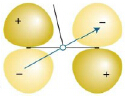
\includegraphics[width=0.9\linewidth]{pig.jpg}\\
			$\pi_g$
		\end{minipage}%
		\begin{minipage}[c]{0.3\linewidth}
			\centering
			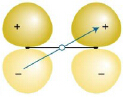
\includegraphics[width=0.9\linewidth]{piu.jpg}\\
			$\pi_u$
		\end{minipage}%
		\begin{minipage}[c]{0.4\linewidth}
			\centering
			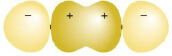
\includegraphics[width=0.9\linewidth]{sigmag.jpg}\\
			$2\sigma_g$\\
			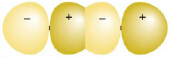
\includegraphics[width=0.9\linewidth]{sigmau.jpg}\\
			$2\sigma_u$
		\end{minipage}\\
		(其中$\pi$ 图示意为 $L_{y/z}$ 本征态, 实际应为环状 $L_x$ 本征态)
	\end{itemize}
\end{itemize}
% subsubsection repr_for_diatom (end)
\subsubsection{成键与反键} % (fold)
\label{ssub:bonding_and_antibonding}
以\ce{H2+} 为例, $r\gg R$ 时
\begin{itemize}
	\item bonding: $\Phi_g = [\psi_{1s}(r_A) + \psi_{1s}(r_B)]/\sqrt{2}$\\
	$E_g - E_{1s}$ 体现出 L-J 势的特征
	\item anti-bonding: $\Phi_u = [\psi_{1s}(r_A) - \psi_{1s}(r_B)]/\sqrt{2}$\\
	$E_u - E_{1s} > 0, E_g - E_{1s}$, 且表现为纯斥力
\end{itemize}
% subsubsection bonding_and_antibonding (end)
\subsubsection{MO 方法} % (fold)
\label{ssub:mo_method}
参照 Hartree-Fock 方法, 基于单电子成键计算多电子的情形: Hund-Mulliken 或者
分子轨道 (molecular orbital (MO)) 方法
\begin{align}
	&\Phi_A = \Phi_g(1)\Phi_g(2)\chi_{0,0}\\
	&\Phi_B = \Phi_u(1)\Phi_u(2)\chi_{0,0}\\
	&\Phi_C = [\Phi_g(1)\Phi_u(2) + \Phi_u(1)\Phi_g(2)]\chi_{0,0}/\sqrt 2\\
	&\Phi_D = [\Phi_g(1)\Phi_u(2) - \Phi_u(1)\Phi_g(2)]\chi_{1,m_s}/\sqrt 2
\end{align}
其中 $\chi_{s,m_s}$ 表示自旋波函数. 四个基分别 $^1\Sigma^+_g$, $^1\Sigma^+_g$, 
$^1\Sigma^+_u$, $^3\Sigma^+_u$

省略自旋波函数, 写为: 
\begin{align}
	&\Phi_A = \Phi_A^{\mathrm{cov}} + \Phi_A^{\mathrm{ion}}\\
	&\Phi_A^{\mathrm{cov}} = \frac 12\left[\psi(r_{1A})\psi(r_{2B})+
		\psi(r_{2A})\psi(r_{1B})\right]\\
	&\Phi_A^{\mathrm{ion}} = \frac 12\left[\psi(r_{1A})\psi(r_{2A})+
		\psi(r_{1B})\psi(r_{2B})\right]
\end{align}
其中 $\psi = \psi_{1s}$. 分离的两式分别表示共价键和离子键. 

于是对于 $^1\Sigma^+_g$ 态, 泛函试探函数写为
\begin{equation}
	\Phi_T = \Phi_A+\lambda\Phi_B = (1-\lambda)\Phi_A^{\mathrm{cov}} 
+ (1+\lambda)\Phi_A^{\mathrm{ion}}
\end{equation}
定义离子键比 $q = (1+\lambda)/(1-\lambda)$ \\
\begin{centering}
	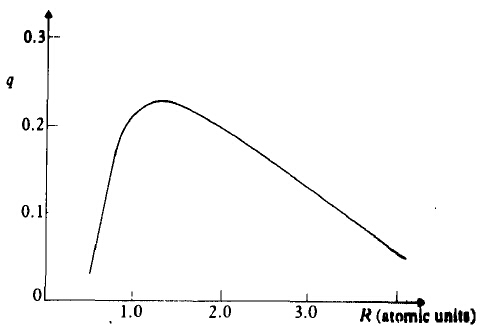
\includegraphics[width=0.9\linewidth]{cov-ion.jpg}
\end{centering}\\
% subsubsection mo_method (end)
其他方法还包括 Heitler-London 或价键方法 (基于 $\Phi_A^{\mathrm{cov}}$ 和
$\Phi_D^{\mathrm{cov}}$). 
\begin{itemize}
	\item 近似方法在势能最低点附近往往偏离 (泛函方法总是偏大) 较多, 因为此时
	离子键, 共价键, 库伦势, 交换势都对于分子势有显著影响
\end{itemize}
% subsection bound (end)
\subsection{长程相互作用} % (fold)
\label{sub:long_range_interaction}
原子 $A$ 和原子 $B$ 的长程相互作用 $R\gg r$
\begin{align}
	& H = H_A + H_B + V\\
	& V = \sum_{ab}\frac{e_a e_b}{\vec R + \vec r_a - \vec r_b}
\end{align}
对于 $V$ 做多极展开
\begin{itemize}
	\item $Q_A, Q_B\neq 0$: $V\sim 1/R$
	\item $Q_A = 0$, $Q_B\neq 0$: $V\sim 1/R^4$
	\item $Q_A = Q_B = 0$: $V$ 的一级微扰消失, 二级 $1/R^6$. (van der Waals 势)
\end{itemize}
% subsection long_range_interaction (end)
% section multibody (end)
\section{散射理论} % (fold)
\label{sec:scattering_theory}
定义: 
\begin{itemize}
	\item 微分散射截面 (differential cross-section): 
	单位时间特定方向上的散射与入射之比
	\begin{equation}
		\sigma(\theta, \varphi) = I(\theta, \varphi) / I
	\end{equation}
	\item 全散射截面 (total cross-section):
	\begin{align}
		\sigma &= \int\sigma(\theta, \varphi)\dif\Omega \\
		&= \int_0^\pi\sin\theta\dif\theta\int_0^{2\pi}\dif\varphi
		\sigma(\theta, \varphi)
	\end{align}
\end{itemize}
设本征波函数分为平面波入射 $\Phi_{\vec k}(\vec r)$ 和球面波散射 $\Phi_s$
\begin{equation}\label{equ:sca_form}
	\Psi(\vec r) \mathop{\sim}_{r\to\infty} \exp(\mi\vec k \cdot \vec r)
	+ f(\theta, \varphi)\frac{\exp(\mi kr)}{r}
\end{equation}
带入波函数流公式 $\vec J = -\mi\hbar\Phi^*\nabla\Phi/2m + \cc$ 
\begin{equation}\label{equ:sca_id}
	\sigma(\theta, \varphi) = |f(\theta, \varphi)|^2
\end{equation}
称 $f(\theta, \varphi)$ 为散射振幅 (scattering amplitude). 对于全同粒子的修正 
(玻色子 $+$, 费米子 $-$)
\begin{equation}
	\sigma(\theta, \varphi) = 
	|f(\theta, \varphi)\pm f(\pi - \theta, \varphi + \pi)|^2 
\end{equation}
\subsection{解的形式与分波法} % (fold)
\label{sub:sol}
\begin{enumerate}
	\item 球坐标下 $(\nabla^2 + k^2)\psi = 0$ 的解
	\begin{equation}
		\psi = j_l(k r)\mathrm Y_l^m(\theta,\varphi) \mbox{~或~}
		n_l(k r)\mathrm Y_l^m(\theta,\varphi)
	\end{equation}
	其中球贝塞尔函数的渐进情况: 
	\begin{align}
		& j_l(x)\mathop{\sim}_{x\to 0} \frac{x^l}{(2l+1)!!}\\
		& n_l(x)\mathop{\sim}_{x\to 0} -\frac{(2l-1)!!}{x^{l+1}}\\
		& j_l(x)\mathop{\sim}_{x\to \infty} \frac 1x
		\sin\left(x-\frac{l\pi}{2}\right)\\
		& n_l(x)\mathop{\sim}_{x\to \infty} \frac 1x
		\cos\left(x-\frac{l\pi}{2}\right)
	\end{align}
	\begin{itemize}
		\item 平面波在球面波上展开
		\begin{equation}\label{equ:plain_on_sphere}
			\e^{ikz} = \sum_{l=1}^\infty (2l+1)\mi^l j_l(kr) 
			\mathrm P_l(\cos\theta)
		\end{equation}
	\end{itemize}
	\item 对于含势 $(\nabla^2 + k^2 - U)\psi = 0$, 解的形式
	\begin{equation}
		\psi = \sum_l C_l \frac 1r F_l(r)\mathrm Y_l^m(\theta, \varphi)
	\end{equation}写
	有径向方程
	\begin{equation}
		\left[\frac{\dif^2}{\dif r^2} - \frac{l(l+1)}{r^2} - U(r) + k^2\right]
		F_l(r) = 0
	\end{equation}
	要求边界 $F_l(0) = 0$. 对于有限势, 无穷远边界
	\begin{equation}\label{equ:radiation_equ}
		F_l(r) \mathop{\sim}_{r\to\infty} 
		\sin\left(kr - \frac{l\pi}{2} + \eta_l\right)
	\end{equation}
	在无穷远出参照 $U=0$ 的结果, 即 (\ref{equ:plain_on_sphere})式, 满足边界
	(\ref{equ:sca_form})式时系数
	\begin{equation}
		C_l = \frac{(2l+1)\mi^l\e^{\mi\eta_l}}{k}
	\end{equation}
	据此有散射振幅和散射截面的表达式
	\begin{align}
		&f(\theta, \varphi) = \frac{1}{k}
		\sum_l (2l+1)\e^{\mi\eta_l}\sin\eta_l\mathrm P_l(\cos\theta) \\
		&\sigma = \frac{4\pi}{k^2}\sum_l (2l+1)\sin^2\eta_l = 
		\frac{4\pi}{k}\Imag f(0)\label{equ:optical_theorem}
	\end{align}
	其中 (\ref{equ:optical_theorem}) 式称为 Optical Theorem
\end{enumerate}
% subsection sol (end)
\subsection{散射长度} % (fold)
\label{sub:scattering_length}
定义 $s$ 波散射长度
\begin{equation}
	a_0 = -\lim_{k\to 0} \frac{\tan\eta_0}{k}
\end{equation}
从而 $s$ 波弹性散射截面 ($k\to 0$)
\begin{equation}
	\sigma_s = \frac{4\pi a^2}{1+k^2a^2}
\end{equation}
对于全同粒子 $k=0$ 时, 根据 (\ref{equ:sca_id})式
\begin{itemize}
	\item 玻色子 $\sigma_s = 8\pi a^2$
	\item 费米子 $\sigma_s = 0$
\end{itemize}
\subsubsection{等效排斥势} % (fold)
\label{ssub:repulsive_potential}
\begin{enumerate}
	\item $U>0$ 时, 总有 $a>0$
	\item $U<0$ 时, 对于不同的势阱深度有 $a>0$ 和 $a<0$
	\begin{itemize}
		\item $a>0$ 表现为排斥????
		\item $a<0$ 表现为吸引????
	\end{itemize}
\end{enumerate}
% subsubsection repulsive_potential (end)
\subsubsection{Quantum defect theory} % (fold)
\label{ssub:quantum_defect_theory}
碱金属对于里德伯定理的修正
\begin{equation}
	E_n = -\frac{Rhc}{n^2} \xlongrightarrow E_n = -\frac{Rhc}{(n-\delta_l)^2}
\end{equation}
来源于原子实-价电子极化以及价电子隧穿入原子实. 用于计算高激发态可以得到结果
\begin{enumerate}
	\item $s$ 波散射的散射长度和最高能级的束缚态能量有关
	\item 最高束缚态能级低于阈值时 $a_0>0$, 反之则高于阈值
	\item 据此可以解释为什么同位素间散射的散射长度与质量数有关
\end{enumerate}
% subsection quantum_defect_theory (end)
% subsection scattering_length (end)
% \subsection{channels 和 thresholds} % (fold)
% \label{sub:channels_thresholds}
% \begin{enumerate}
% 	\item channels: $A+B\xlongrightarrow A' + B'$ 中, $A$ 和 $B$ 
% 	散射前后状态的描述. 对于弹性散射, channel 不变. 守恒率允许的称为 open 
% 	channel, 反之 closed channel
% 	\item thresholds (对于非弹性散射) 质心系下允许反应发生的最小能量
% \end{enumerate}
% subsection channels_thresholds (end)
\subsection{Feshbach 共振} % (fold)
\label{sub:feshbach_resonance}
通过调整外场影响原子-原子相互作用, 从而改变散射长度.
\begin{enumerate}
	\item magnetic Feshbach 共振: \\
	\begin{centering}
		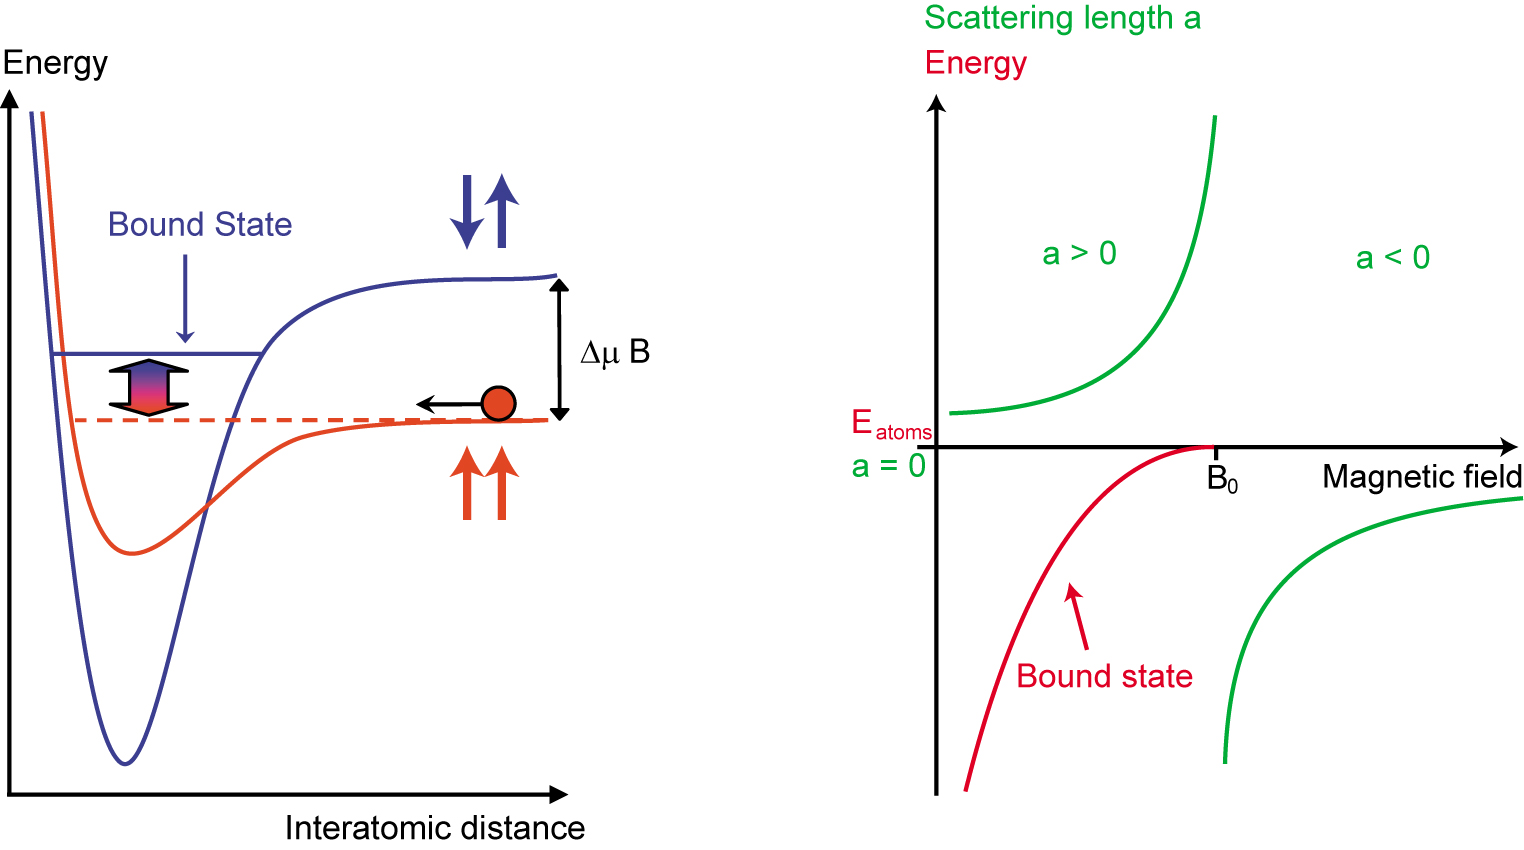
\includegraphics[width = \linewidth]{Feshbach.jpg}
	\end{centering}
	在产生束缚态的磁场附近, 散射长度 $a$ 出现奇点 ($\eta \approx \pi/2$), 
	从而较小的磁场调节范围能显著改变散射长度. 对于费米子体系, 不同散射长度下, 
	同时产生分子 BEC 到原子 BCS 转换\\
	\begin{centering}
		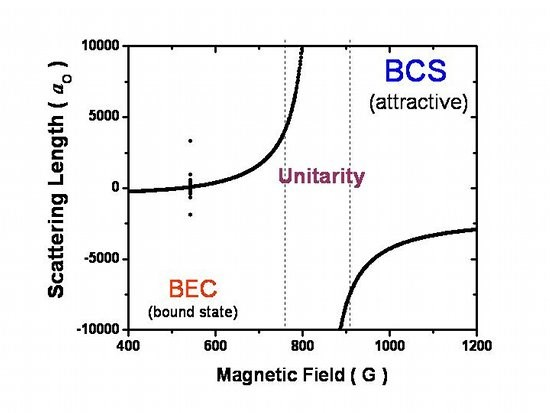
\includegraphics[width=\linewidth]{bec_bcs.jpg}
	\end{centering}
	\item optical Feshbach 共振\\
	\begin{centering}
		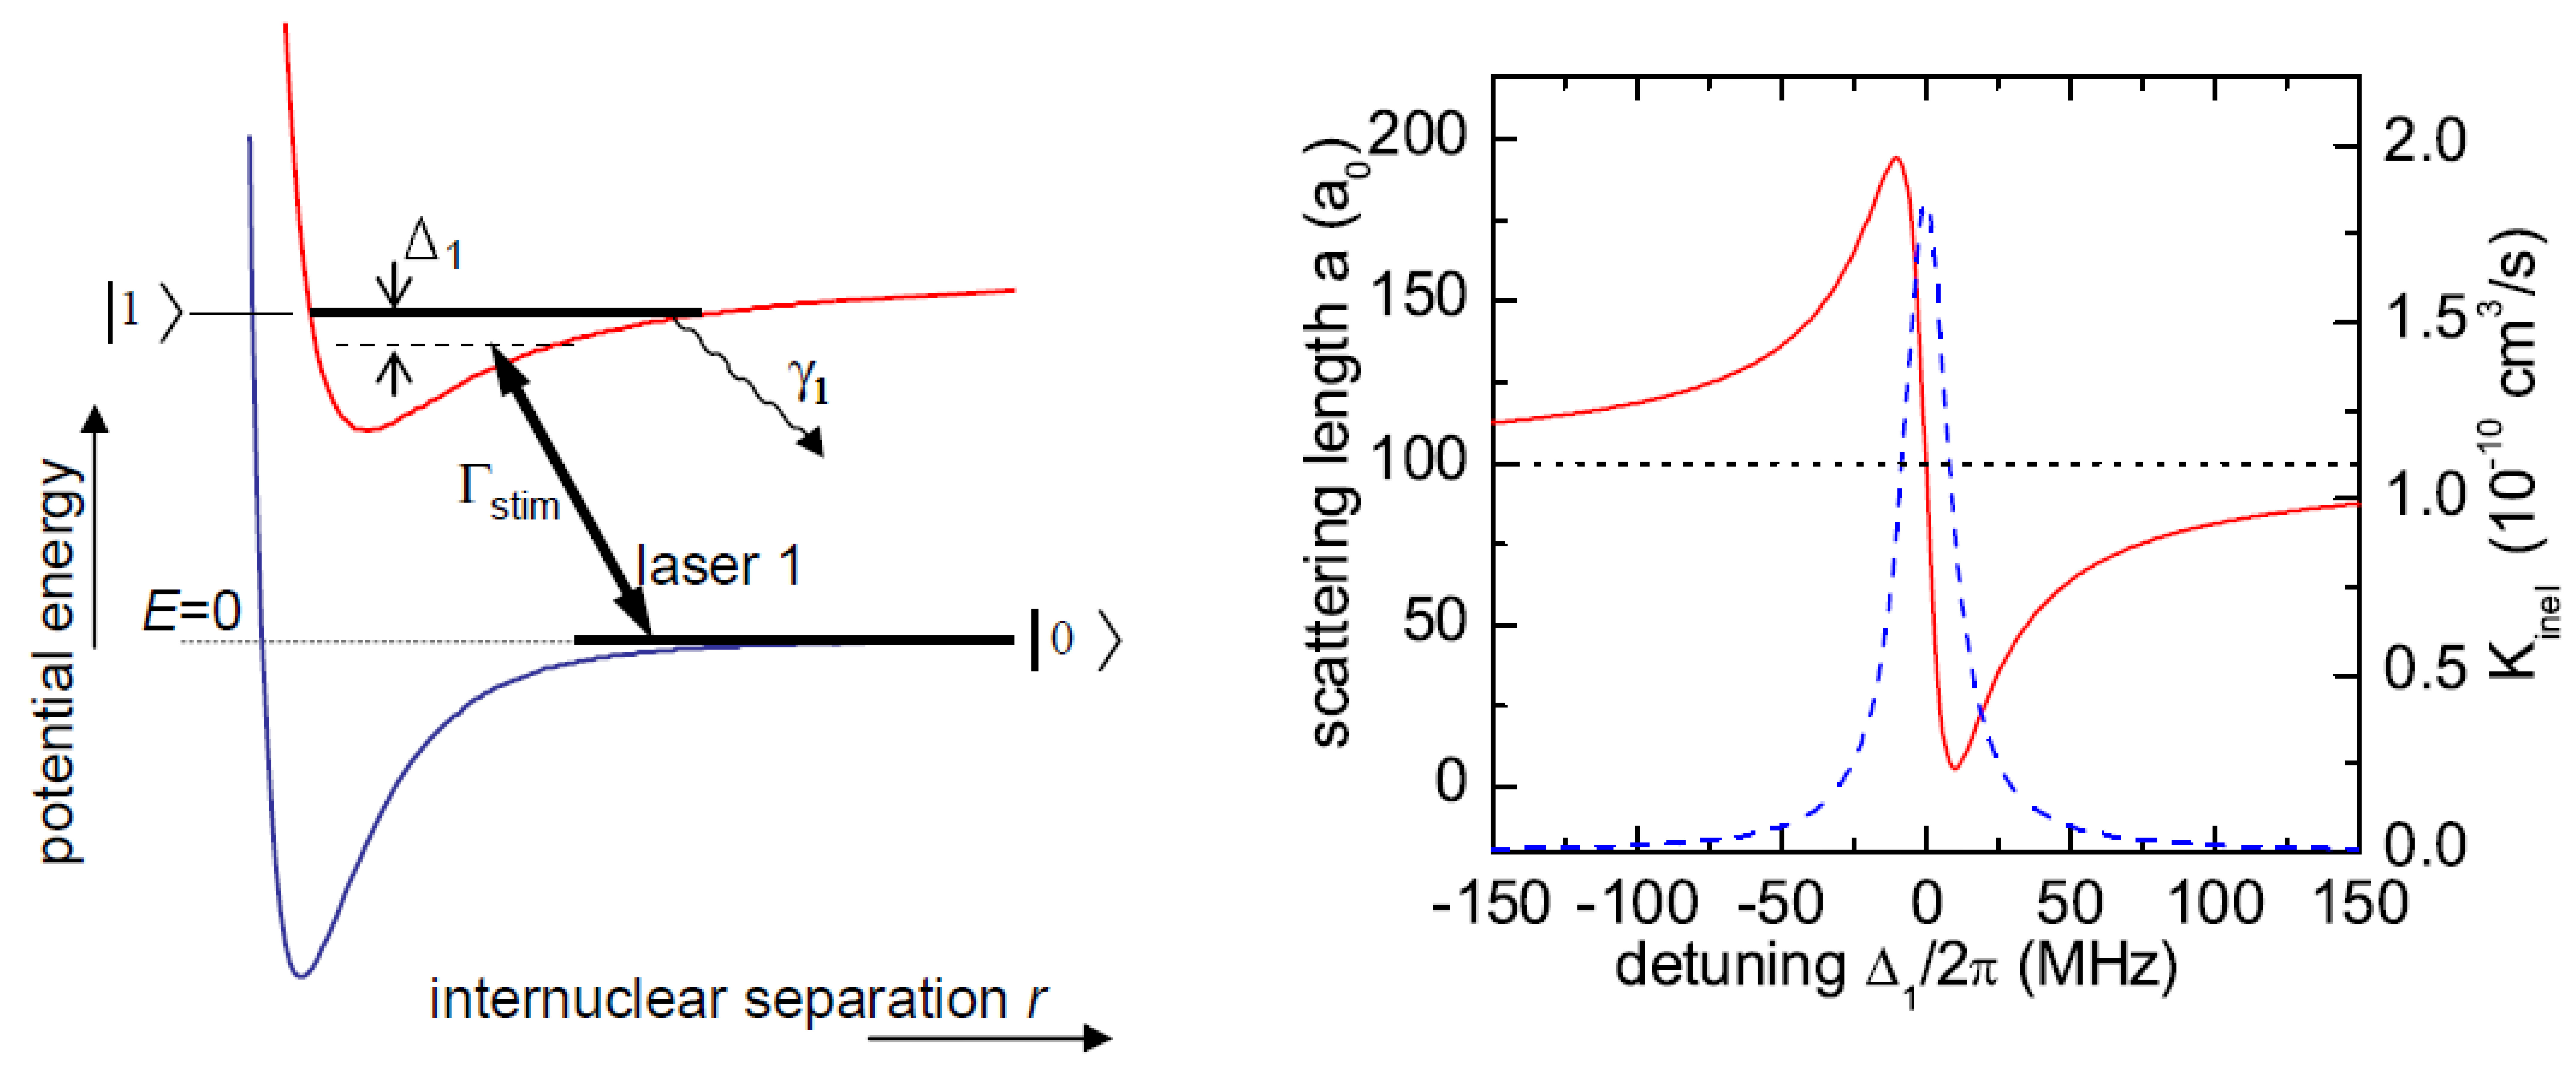
\includegraphics[width=\linewidth]{ofr.jpg}
	\end{centering}
\end{enumerate}
% subsection feshbach_resonance (end)
\subsection{shape resonance (optential resonance)} % (fold)
\label{sub:shape_resonance}
shape resonance (optential resonance): 
由于势能曲线中有势垒而产生的准束缚态 (亚稳)\\
\begin{centering}
	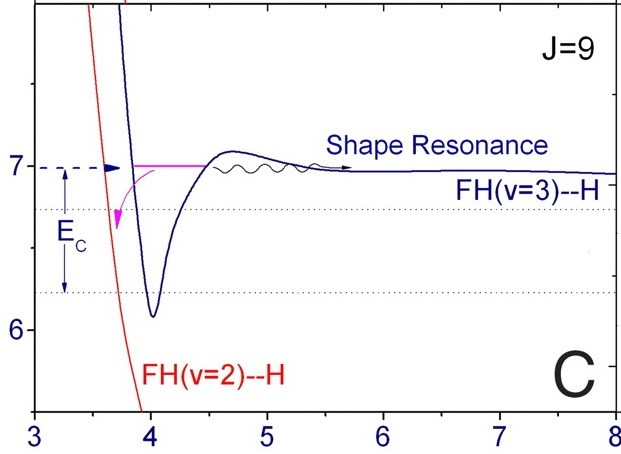
\includegraphics[width=\linewidth]{shape-res.jpg}
\end{centering}\\
当亚稳态被破坏时, 内部状态不变.
% subsection shape_resonance (end)
% section scattering_theory (end)
\section*{鸣谢} 
本文档参考郑盟锟老师的讲义, 由唐如麟校对
\end{document}